\documentclass[twoside,numbers,spanish]{ezthesis}
%% # Opciones disponibles para el documento #
%%
%% Las opciones con un (*) son las opciones predeterminadas.
%%
%% Modo de compilar:
%%   draft            - borrador con marcas de fecha y sin im'agenes
%%   draftmarks       - borrador con marcas de fecha y con im'agenes
%%   final (*)        - version final de la tesis
%%
%% Tama'no de papel:
%%   letterpaper (*)  - tama'no carta (Am'erica)
%%   a4paper          - tama'no A4    (Europa)
%%
%% Formato de impresi'on:
%%   oneside          - hojas impresas por un solo lado
%%   twoside (*)      - hijas impresas por ambos lados
%%
%% Tama'no de letra:
%%   10pt, 11pt, o 12pt (*)
%%
%% Espaciado entre renglones:
%%   singlespace      - espacio sencillo
%%   onehalfspace (*) - espacio de 1.5
%%   doublespace      - a doble espacio
%%
%% Formato de las referencias bibliogr'aficas:
%%   numbers          - numeradas, p.e. [1]
%%   authoryear (*)   - por autor y a'no, p.e. (Newton, 1997)
%%
%% Opciones adicionales:
%%   spanish         - tesis escrita en espa'nol
%%
%% Desactivar opciones especiales:
%%   nobibtoc   - no incluir la bibiolgraf'ia en el 'Indice general
%%   nofancyhdr - no incluir "fancyhdr" para producir los encabezados
%%   nocolors   - no incluir "xcolor" para producir ligas con colores
%%   nographicx - no incluir "graphicx" para insertar gr'aficos
%%   nonatbib   - no incluir "natbib" para administrar la bibliograf'ia

%% Paquetes adicionales requeridos se pueden agregar tambi'en aqu'i.
%% Por ejemplo:
%\usepackage{subfig}
%\usepackage{multirow}
\usepackage{amssymb,amsmath,alltt}
\usepackage[utf8]{inputenc} % Escribir con acentos, n, ...
\usepackage[spanish]{babel}
%\usepackage[activeacute,spanish]{babel}
%\renewcommand\shorthandsspanish{}
\usepackage{graphicx}
\usepackage{setspace}
%\usepackage{epsfig}
\usepackage[absolute]{textpos}
\usepackage[colorinlistoftodos]{todonotes}
\usepackage{xfrac}
\usepackage{lmodern}
\usepackage{enumerate}
\usepackage{babelbib}
%\usepackage{natbib}
\usepackage{relsize}
%\usepackage{amsfonts}
%\usepackage{bbold}
\usepackage{dsfont}
\usepackage{bm}
\usepackage{slashed}
\usepackage{tensor}
\newtheorem{example}{Ejemplo}
\let\mathbb\mathds
\DeclareMathOperator{\Tr}{Tr}
\makeatletter
\def\@xfootnote[#1]{%
  \protected@xdef\@thefnmark{#1}%
  \@footnotemark\@footnotetext}
\makeatother

%% # Datos del documento #
%% Nota que los acentos se deben escribir: \'a, \'e, \'i, etc.
%% La letra n con tilde es: \~n.

%\author{Juan Antonio Navarro P\'erez}
%\title{Ejemplo de una Tesis}
%\degree{Doctor en Ciencias}
%\supervisor{Nombre de mi Asesor}
%\institution{Universidad de Alg\'un Sitio}
%\faculty{Escuela de Ingenier\'ia y Ciencias}
%\department{Departamento de Sistemas Computacionales}

%% # M'argenes del documento #
%% 
%% Quitar el comentario en la siguiente linea para austar los m'argenes del
%% documento. Leer la documentaci'on de "geometry" para m'as informaci'on.

%\geometry{top=40mm,bottom=33mm,inner=40mm,outer=25mm}
\geometry{lmargin=2.5cm,rmargin=2.5cm,tmargin=3cm,bmargin=3cm}
\parskip= 6pt

%% El siguiente comando agrega ligas activas en el documento para las
%% referencias cruzadas y citas bibliogr'aficas. Tiene que ser *la 'ultima*
%% instrucci'on antes de \begin{document}.
\hyperlinking
\begin{document}

%% En esta secci'on se describe la estructura del documento de la tesis.
%% Consulta los reglamentos de tu universidad para determinar el orden
%% y la cantidad de secciones que debes de incluir.

%% # Portada de la tesis #
%% Mirar el archivo "titlepage.tex" para los detalles.

\pagenumbering{roman} \setcounter{page}{1}

%%
%% Esqueleto para la portada de las tesis para
%% la Facultad de Ciencias de la UNAM
%%


%%%%%%%%%%%%%%%%%%%%%%%%%%%%%%%%%%%%%%%%%%%%%%%%%%%%%%%
%% Comandos para la portada

\newcommand{\titulo}[1]{\def\eltitulo{#1}}
%* lacarrera corresponde al tí­tulo otorgado -Matemático-
%* NO AL NOMBRE DE LA CARRERA -Matemáticas- --RRP
\newcommand{\carrera}[1]{\def\lacarrera{#1}}
\newcommand{\nombre}[1]{\def\elnombre{#1}}    %* Del alumno
\newcommand{\director}[1]{\def\eldirector{#1}}  %* De tesis
\newcommand{\fecha}[1]{\def\lafecha{#1}}

%% Llena los siguientes datos (usa MAYÚSCULAS)
%%Estos datos aparecerán en la portada y los encabezados
\titulo{TÍTULO TENTATIVO}
\nombre{\uppercase{ARTURO ALONSO SANTAELLA ORTEGA}}
\carrera{FÍSICO}
\director{\uppercase{Dr. Jaime Besprosvany Fridzon}}
\fecha{México, D.F. 2016}

\thispagestyle{empty}

%% Barra izquierda - Escudos
\hskip-1.5cm
\begin{minipage}[c][10cm][s]{3cm} 
  \begin{center}
    
\includegraphics[height=2.6cm]{escudo-unam.jpg}\\[10pt]
    \hskip2pt\vrule width2pt height13cm\hskip1mm
    \vrule width1pt height13cm\\[10pt]
    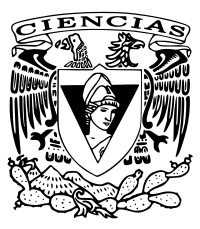
\includegraphics[height=2.6cm]{escudo_ciencias.png}
  \end{center}
\end{minipage}\quad
%% Barra derecha - Tí­tulos
\begin{minipage}[c][9.5cm][s]{10cm}
  \begin{center}
    % Barra superior
    {\large \scshape Universidad Nacional Aut\'onoma de M\'exico}
    \vspace{.3cm}
    \hrule height2pt
    \vspace{.1cm}
    \hrule height1pt
    \vspace{.3cm}
    {\scshape Facultad de Ciencias}

    % Titulo del trabajo
    \vspace{3cm}

    {\Large \eltitulo}

    \vspace{3cm}

    % Tipo de trabajo
    \makebox[8cm][s]{\Huge T E S I S}\\[8pt]
    QUE PARA OBTENER EL T\'ITULO DE:\\[3pt]
    \mbox{}\lacarrera\\[13pt]
    PRESENTA:\\[3pt]
    \elnombre

    \vspace{2cm}

    {\small DIRECTOR DE TESIS:\\ \eldirector}

    \vspace{2cm}

    \lafecha
    
  \end{center}
\end{minipage}





%% # Prefacios #
%% Por cada prefacio (p.e. agradecimientos, resumen, etc.) crear
%% un nuevo archivo e incluirlo aqu'i.
%% Para m'as detalles y un ejemplo mirar el archivo "gracias.tex".
%%% Las secciones del "prefacio" inician con el comando \prefacesection{T'itulo}
%% Este tipo de secciones *no* van numeradas, pero s'i aparecen en el 'indice.
%%
%% Si quieres agregar una secci'on que no vaya n'umerada y que *tampoco*
%% aparesca en el 'indice, usa entonces el comando \chapter*{T'itulo}
%%
%% Recuerda que aqu'i ya puedes escribir acentos como: 'a, 'e, 'i, etc.
%% La letra n con tilde es: 'n.

\prefacesection{Agradecimientos}

Este trabajo no habr'ia sido posible sin el apoyo y el est'imulo de mi colega
y amigo, Doctor Rudolf Fliesning,  bajo cuya supervisi'on escog'i este tema y
comenc'e la tesis. Sr. Quentin Travers, mi consejero en las etapas finales
del trabajo, tambi'en ha sido generosamente servicial, y me ha ayudado de
numerosos modos, incluyendo el resumen del contenido de los documentos que
no estaban disponibles para mi examen, y en particular por permitirme leer, 
en cuanto estuvieron  disponibles, las copias de los  recientes extractos de
los diarios de campa'na del Vigilante Rupert Giles y la actual Cazadora la
se'norita Buffy Summers, que se encontraron con William the Bloody en 1998, y
por facilitarme el pleno acceso  a los diarios de anteriores Vigilantes
relevantes a la carrera de William the Bloody.

Tambi'en me gustar'ia agradecerle al Consejo la concesi'on de Wyndham-Pryce
como Compa'nero, el cual me ha apoyado durante mis dos a'nos de investigaci'on,
y la concesi'on de dos subvenciones de viajes, una para estudiar documentos
en los Archivos de Vigilantes sellados en Munich, y otra para la
investigaci'on en campa'na en Praga. Me gustar'ia agradecer a Sr. Travers,
otra vez, por facilitarme  la acreditaci'on  de seguridad para el trabajo en
los Archivos de Munich, y al Doctor Fliesning por su apoyo colegial y ayuda
en ambos viajes de investigaci'on.

No puedo terminar sin agradecer a mi familia, en cuyo est'imulo constante y
amor he confiado a lo largo de mis a'nos en la Academia. Estoy agradecida
tambi'en a los ejemplos de mis  difuntos hermano, Desmond Chalmers, Vigilante
en Entrenamiento, y padre, Albert Chalmers, Vigilante. Su coraje resuelto
y convicci'on siempre me inspirar'an, y espero seguir, a mi propio y peque'no
modo, la noble misi'on por la que dieron sus vidas. Es a ellos a quien dedico
este trabajo.

%% Por si alguien tiene curiosidad, este "simp'atico" agradecimiento est'a
%% tomado de la "Tesis de Lydia Chalmers" basada en el universo del programa
%% de televisi'on Buffy, la Cazadora de Vampiros.
%% http://www.buffy-cazavampiros.com/Spiketesis/tesis.inicio.htm


%% # 'Indices y listas de contenido #
%% Quitar los comentarios en las lineas siguientes para obtener listas de
%% figuras y cuadros/tablas.
\tableofcontents
%\listoffigures
%\listoftables

\pagenumbering{arabic} \setcounter{page}{1}
%\setcounter{chapter}{-1}
%% # Cap'itulos #
%% Por cada cap'itulo hay que crear un nuevo archivo e incluirlo aqu'i.
%% Mirar el archivo "intro.tex" para un ejemplo y recomendaciones para
%% escribir.
%%% Los cap'itulos inician con \chapter{T'itulo}, estos aparecen numerados y
%% se incluyen en el 'indice general.
%%
%% Recuerda que aqu'i ya puedes escribir acentos como: 'a, 'e, 'i, etc.
%% La letra n con tilde es: 'n.

\chapter{Introducci'on}

Existen dos tipos de citas bibliograf'icas: usa \verb|\citep{..}| para
citas en \emph{par'entesis} y \verb|\citet{..}| para citas
en el \emph{texto}. Por ejemplo, estudios reciente han mostrado nuevos e
interesantes modelos que se pueden aplicar para reformular teor'ias
f'isicas~\citep{NewCam97}. Mientras que, el trabajo de \citet{Rofl06} fue
considerado muy divertido por una significativa fracci'on de la comunidad
de investigadores. Tambi'en es posible citar a varios trabajos en una sola
referencia \citep{Lamport86,Knuth84}.

Estos comandos para producir citas bibliograficas son provistos por
el paquete \textsf{natbib}. Para obtener m'as informaci'on, consulta la
documentaci'on de ese paquete~\citep{doc:natbib}. Por su parte, en
la documentaci\'on de \textsf{geometry} puedes encontrar detalles
adicionales sobre el sistema para ajustar los m'argenes del
documento~\citep{doc:geometry}. Lo que sigue
es un mont'on de texto sin sentido en lat'in que utilizaremos para llenar
algunas p'aginas.

Lorem ipsum dolor sit amet, consectetuer adipiscing elit. Integer arcu nisl,
consectetuer ut, vehicula nec, blandit id, nulla. Vestibulum in odio a odio
volutpat sollicitudin. Donec congue porta tellus. Ut quis est sed velit
blandit fringilla. Nunc lobortis dui vitae sapien. In tincidunt magna eget
purus. Nam lorem quam, vehicula in, dictum et, congue eget, odio. Curabitur
gravida mi id dui. Aliquam erat volutpat. Fusce velit turpis, accumsan vel,
tincidunt at, aliquet at, sem. Cras viverra eros ac orci. Aenean vestibulum,
lorem sed luctus congue, arcu pede ultricies libero, at posuere felis nulla
et leo.

Fusce rhoncus lobortis orci. Quisque suscipit dolor. In tincidunt dictum
elit. Cras metus. Donec nibh mi, ornare a, ullamcorper in, gravida non,
augue. Aliquam erat volutpat. Aliquam commodo tellus sed dolor. Sed urna.
Phasellus blandit orci sit amet nulla. Fusce vel eros. Aenean ultrices
sodales mi. Aliquam erat volutpat. Fusce orci sem, sollicitudin convallis,
auctor a, sollicitudin vitae, dui. Sed massa. Duis luctus lectus ut lacus.

Morbi felis tellus, placerat quis, congue pretium, consectetuer at, tortor.
Nunc condimentum mattis urna. Donec dolor erat, fringilla ut, auctor ac,
vestibulum ut, velit. Aliquam convallis magna ac neque. Praesent varius
congue augue. Nulla adipiscing urna faucibus diam. Mauris porta sapien ut
justo. Donec suscipit tortor gravida ligula. Aliquam ac purus et massa
scelerisque vehicula. Maecenas a libero. Class aptent taciti sociosqu ad
litora torquent per conubia nostra, per inceptos himenaeos. Pellentesque
sit amet est eget metus tincidunt semper. Phasellus nec purus. Proin
venenatis lectus vel elit. Pellentesque augue quam, tincidunt sed, pretium
ut, feugiat id, odio. Aenean eu nibh et quam dignissim facilisis.

Suspendisse adipiscing. Maecenas tincidunt placerat justo. Ut mattis nunc ac
orci. Vestibulum quis velit sed massa vulputate posuere. Duis rhoncus lacus.
Quisque non lacus et nibh molestie tincidunt. Nulla tortor pede, auctor id,
eleifend sit amet, ultrices id, risus. Duis et lectus. Suspendisse interdum,
magna ut porta porta, quam tellus suscipit ligula, cursus consectetuer purus
erat et dolor. Phasellus venenatis, risus malesuada lacinia placerat, lectus
tellus lobortis ligula, eu porttitor tellus nibh eu enim. Morbi vel erat in
sem pharetra molestie. Duis tellus. In ipsum. Vivamus ac augue sed dui
hendrerit pulvinar. In dui erat, molestie ut, lacinia at, sagittis sed, nisi.
Maecenas libero. Nam volutpat dictum erat.

Fusce laoreet sapien ut lorem. Mauris sed leo a mi luctus sollicitudin.
Donec ornare nisi id dolor. Ut eros metus, tristique quis, ultrices ac,
accumsan cursus, est. Pellentesque mollis posuere sapien. Morbi nec augue.
Cum sociis natoque penatibus et magnis dis parturient montes, nascetur
ridiculus mus. Duis tristique, ipsum in tincidunt gravida, nunc nulla
vehicula felis, elementum eleifend nunc elit id magna. Cum sociis natoque
penatibus et magnis dis parturient montes, nascetur ridiculus mus. Curabitur
rhoncus dui ut sapien.

Sed orci. Nunc nisi lorem, convallis nec, porttitor at, porttitor et, erat.
Lorem ipsum dolor sit amet, consectetuer adipiscing elit. Donec luctus, velit
quis lacinia pulvinar, risus urna malesuada nisl, vel hendrerit erat enim ac
enim. Aliquam sapien dolor, fringilla quis, consequat auctor, sodales id,
est. In imperdiet est et dui. Cras libero lacus, feugiat a, auctor ut,
vulputate sollicitudin, orci. Ut tellus velit, rutrum tristique, eleifend sit
amet, auctor consectetuer, sapien. Fusce eget justo. Nam auctor lorem at
purus. Vestibulum ante ipsum primis in faucibus orci luctus et ultrices
posuere cubilia Curae; Pellentesque pretium enim sed tortor. Sed luctus velit
at ligula. Nunc id elit. Curabitur lacus. Mauris placerat nibh sit amet
turpis. Fusce varius, justo et ultrices dictum, urna risus rhoncus ipsum, sed
ultricies nunc arcu eu risus. Nam vitae purus.

Proin augue. Duis vehicula mauris sollicitudin sapien. Nam tristique lacus
nec nisl. Praesent quis enim. Vestibulum vel velit in purus luctus mattis.
Mauris ullamcorper tempor lorem. Quisque rutrum. Praesent enim nibh,
pellentesque non, lacinia accumsan, euismod a, lorem. Etiam fringilla
iaculis mauris. Aenean adipiscing purus in lacus. Maecenas quis nibh. Ut
non augue at mauris elementum luctus. Duis varius tincidunt mi. Aliquam
justo massa, auctor nec, malesuada interdum, mollis ac, mauris. Maecenas
ultricies gravida dui. Aliquam arcu elit, pretium eu, gravida ac, molestie
eu, enim. Etiam facilisis orci eget est. Integer eu orci non felis tincidunt
consectetuer. Sed imperdiet ultrices nibh.

\chapter*{Notación}
\label{chap:NOT}
\addcontentsline{toc}{chapter}{Notación}

\small{
\noindent A continuación se presenta un listado de las convenciones de notación, signo, etc., utilizadas en el presente texto, con el objetivo de eliminar ambigüedades asociadas a la multiplicidad de éstas en actual utilización en la literatura del tema. 
\begin{itemize}

	\item (\textit{Unidades naturales}) Se utilizan unidades tales que $\hbar=c=1$, siendo las primeras secciones del capítulo 1 la excepción a esta regla.

	\item La métrica de Minkowski es:
	\begin{equation*} 
		g^{\mu\nu}=	\begin{pmatrix}
					1 & 0 & 0 & 0 \\
					0 & -1 & 0 & 0 \\
					0 & 0 & -1 & 0 \\
					0 & 0 & 0 & -1 \\
					\end{pmatrix},
	\end{equation*}
	
	\noindent en coincidencia con \citep{Itzykson}, \citep{Bjorken} y \citep{GreinerRQM}, por ejemplo, pero en discrepancia con \citep{Lurie}, \citep{RobinsonSymmetry} y \citep{WeinbergQTF}. Además, $g^{\mu \nu}=g_{\mu \nu}=(g^{-1})^{\mu \nu}$.
	
	\item Índices en letras latinas (e.g. $i$, $j$, $k$, etc.) toman valores en $\{1,2,3\}$ mientras que índices en letras griegas (e.g. $\alpha$, $\beta$, $\mu$, $\nu$, etc.) toman valores en $\{0,1,2,3\}$. Excepciones a lo anterior se harán explícitas.

	\item (\textit{Convención de suma de Einstein}) Se suma sobre parejas de índices repetidos en una misma expresión (e.g. $u_\alpha v^{\alpha} \equiv \sum_\alpha u_\alpha v^{\alpha} $). Excepciones a lo anterior se harán explícitas. 
	
	\item Los vectores contravariantes se escriben con índices arriba: $x^{\mu}=(x^0,x^1,x^2,x^3)$; los vectores covariantes con índices abajo: $x_{\mu}=(x_0,x_1,x_2,x_3)=(x^0,-x^1,-x^2,-x^3)=g_{\mu \nu}x^{\nu}$. La 4-posición y el 4-momento son: $x^{\mu}=(x^0,x^1,x^2,x^3)=(t,x,y,z)=(t,\mathbf{x})$ y $p^{\mu}=(p^0,p^1,p^2,p^3)=(E,p_x,p_y,p_z)=(E,\mathbf{p})$, respectivamente. 
	
	\item Se define $\partial_\mu=\frac{\partial}{\partial x^{\mu}}$, con lo cual $\partial^2=\partial_\mu \partial^{\mu}= \frac{\partial^2}{\partial t^2}-\nabla^2$ es el operador D\textquotesingle Alambertiano; el \textit{operador} de 4-momento es: $\hat{p}^\mu= i\partial^\mu=i\frac{\partial}{\partial x_\mu}=(i\frac{\partial}{\partial t},-i\mathbf{\nabla})=(\hat{E},\mathbf{\hat{p}})$.
	
\end{itemize}
}

\chapter{Mecánica cuántica relativista}
\label{chap:MCR}

\section{Introducción}
\label{sec:IntroMCR}

La descripción de fenómenos físicos a altas energías requiere de una teoría cuántica consistente con la relatividad especial. La transición de una teoría no relativista a la relativista requiere de la re-formulación de algunos conceptos en la teoría no relativista, en particular:
\begin{enumerate}
	\item Las coordenadas temporales y espaciales deben ser tratadas de manera equivalente. Lo anterior no sucede en la en la mecánica cuántica no-relativista al aparecer $\frac{\partial}{\partial t}$ pero no $\overline{\nabla}$, sino $\nabla^2$ en la ecuación de Schrödinger.
	\item El principio de incertidumbre de Heisenberg implica que si la posición de una partícula es incierta entonces también el tiempo y la energía lo son:
	$$\Delta t\sim \frac{\Delta x}{c}\sim \frac{\hbar}{2c\Delta p }\sim \frac{\hbar}{2mc^2};$$ la posición de una partícula no puede ser determinada 
	con mayor precisión que su longitud de onda de Compton $\lambda_c=\frac{\hbar}{mc}$, de otro modo $E>2mc^2$ y se presenta la creación y aniquilación de pares.

	\item A energías relativistas se presenta la creación y aniquilación de partículas en pares de partícula y antipartícula, por lo que la conservación del número de partículas deja de ser válida. Lo anterior ocurre, por ejemplo, para partículas moviéndose a velocidades comparables a la velocidad de la luz.
\end{enumerate}

Como primer paso en la introducción de una teoría cuántica relativista seguimos el proceso histórico comenzando con el estudio de ecuaciones de onda relativistas de una partícula, i.e. ecuaciones de onda invariantes ante transformaciones de Lorentz\footnote{Éstas se introducen propiamente en la sección (\ref{sec:CovED})}.
%%%%%%%%%%%%%%%%%%%%%%%%%%%%%%%%%%%%%%%%%%%%%%%%%%%%%%%%%%%%%%%%%%%%%%%%%%%%%%%%%%%%%%%%%%%%%%%%%%%%%%%%%%%%%%
%%%%%%%%%%%%%%%%%%%%%%%%%%%%%%%%%%%%%%%%%%%%%%%%%%%%%%%%%%%%%%%%%%%%%%%%%%%%%%%%%%%%%%%%%%%%%%%%%%%%%%%%%%%%%%
\section{Ecuación de Klein-Gordon}
\label{sec:EcKleinGordon}

La energía clásica de una partícula no relativista con masa $m$, posición $\mathbf{x}$ y momento $\mathbf{p}$, sujeta a un potencial $V(\mathbf{x})$ es
\begin{equation}\label{EnergiaClasica}
\begin{array}{rl}
E&=H\\
&=\dfrac{\mathbf{p}^2}{2m}+V(\mathbf{x}).
\end{array}
\end{equation}
La ecuación (\ref{EnergiaClasica}) encapsula la dinámica entera del sistema; la utilización del formalismo apropiado ---i.e. Newton, Lagrange, Hamilton--- permite la determinación de $\mathbf{x}$ y $\mathbf{v}$, tras lo cual el sistema queda completamente descrito.\footnotemark
\footnotetext{En general $\mathbf{q}$ y $\dot{\mathbf{q}}$, ó $\mathbf{q}$ y $\mathbf{p}$.}

En la mecánica cuántica no-relativista un sistema ha sido enteramente descrito cuando se conoce $\Psi(\mathbf{x})$, solución de la \textit{ecuación de onda de Schrödinger}:
\begin{equation}\label{eq:Schrodinger}
i\hbar\frac{\partial}{\partial t}\Psi(\mathbf{x},t)=\left( -\frac{\hbar^2}{2m}\nabla^2 +V(\mathbf{x},t)\right)\Psi(\mathbf{x},t).
\end{equation}

La ecuación de Schrödinger (\ref{eq:Schrodinger}) puede también considerarse una consecuencia de (\ref{EnergiaClasica}) si en ésta se efectúa la siguiente transcripción operadores:
\begin{equation}\label{eq:TransOperadores}
\begin{array}{rl}
E\rightarrow \hat{E}&=i\hbar\dfrac{\partial}{\partial t}, \\[4pt] 
\mathbf{p}\rightarrow\hat{\mathbf{p}}&=-i\hbar\bar{\nabla}, \\[3.5pt]
H\rightarrow \hat{H}&=\dfrac{\hat{\mathbf{p}}^2}{2m}+V(\mathbf{x}).\\ 
\end{array}
\end{equation}

La mecánica descrita por (\ref{EnergiaClasica})---y en consecuencia por (\ref{eq:Schrodinger})--- es claramente no-relativista: basta observar que $E$ y $\mathbf{p}$ no aparecen en igualdad de condiciones; los distintos órdenes de las derivadas evidencain que esta expresión no puede ser invariante ante transformaciones de Lorentz. Lo anterior sugiere la posibilidad de obtener una ecuación de onda invariante ante transformaciones de Lorentz (de ahora en adelante, \textit{Lorentz-covariante}) partiendo de una relación relativista para la energía análoga a (\ref{EnergiaClasica}). De acuerdo con la relatividad especial, la energía de una partícula relativista libre de masa $m$ está dada por
\begin{equation}\label{EnergiaRel}
p^{\mu} p_{\mu} =\frac{E^2}{c^2}-\mathbf{p}\cdot\mathbf{p}=m^2c^2.
\end{equation}
Al sustituir $p^\mu$ por el operador de 4-momento $\hat{p}^\mu$,
\begin{equation}\label{Op4Momento}
\hat{p}^\mu =\left(\hat{p}_0,\hat{\mathbf{p}} \right)=
i\hbar\left( \dfrac{\partial}{\partial(ct)},-\dfrac{\partial}{\partial x},-\dfrac{\partial}{\partial y},-\dfrac{\partial}{\partial z} \right)
\end{equation}
se obtiene la ecuación de \textit{Klein-Gordon} para una partícula libre:
\begin{equation}\label{EcKleinGordon1}
\left( \hat{p}^\mu \hat{p}_\mu -m^2c^2\right)\psi=0.
\end{equation}
Es posible reescribir (\ref{EcKleinGordon1}) con la ayuda de (\ref{Op4Momento}) para obtener
\begin{equation}\label{EcKleinGordon2}
\left( \frac{\partial^2}{c^2 \partial t^2} -\frac{\partial^2}{\partial x^2}-\frac{\partial^2}{\partial y^2}-\frac{\partial^2}{\partial z^2}+\frac{m^2c^2}{\hbar^2} \right)\psi \equiv \left( \Box+\frac{m^2 c^2}{\hbar^2}\right) \psi=0.
\end{equation}
Se verifica de inmediato la Lorentz-covariancia de (\ref{EcKleinGordon1}) y (\ref{EcKleinGordon2}) al ser $\hat{p}^\mu\hat{p}_\mu$ Lorentz-covariante. 
Las soluciones libres de la ecuación de Klein-Gordon son ondas planas de la forma
\begin{equation}\label{SolLibKG}
\psi=N\exp{\left( -\frac{i}{\hbar}p_\mu x^\mu\right)}=N\exp{\left[ \frac{i}{\hbar}(\mathbf{p}\cdot \mathbf{x}-Et)\right]},
\end{equation}
con $N$ una constante de normalización. La inserción de (\ref{SolLibKG}) en la ecuación de Klein-Gordon arroja la relación
\begin{equation*}
p^{\mu}p_{\mu}=\frac{E^2}{c^2}-\mathbf{p}^2=m^2c^2, 
\end{equation*}
de donde
\begin{equation}\label{EnergiaKG}
 E=\pm \sqrt{m^2 c^4+\mathbf{p}^2c^2}.
\end{equation}

Lo anterior muestra que la ecuación de Klein-Gordon admite soluciones con energía tanto positiva como negativa. Las soluciones con energía negativa inicialmente representaron un obstáculo para la teoría, no obstante, éstas fueron posteriormente interpretadas con éxito en términos de antipartículas al reinterpretar (\ref{EcKleinGordon1}) en el marco de una teoría cuántica de campos.

Finalmente, se hace notar que es posible la construcción de una 4-corriente $j^\mu$:
\begin{equation}\label{CorrienteKG}
 j^\mu=(c\rho,-\mathbf{j})=\frac{i\hbar}{2m}(\psi^* \partial^\mu \psi-\psi \partial^\mu \psi^*),
\end{equation}
asociada a la ecuación de onda (\ref{EcKleinGordon1}), que de manera análoga al caso no relativista satisface
\begin{equation}\label{ContinuidadKG}
 \partial_\mu j^\mu=\frac{\partial \rho}{\partial t}+\nabla\cdot \mathbf{j}=0.
\end{equation}

%En (\ref{CorrienteKG}) y (\ref{ContinuidadKG}) $\partial_\mu\equiv\frac{\partial}{\partial x^\mu}$. 
La identidad (\ref{ContinuidadKG})  sugiere naturalmente 
la posibilidad de interpretar $\rho$ como una densidad de probabilidad; esta interpretación resulta imposible al observar que $\psi$ y $\frac{\partial \psi}{\partial t}$ 
pueden tomar valores arbitrarios, con lo cual $\rho$ no satisface ser positivo-definida. Esta situación, así como las antes mencionadas soluciones de energía negativa motivaron 
la búsqueda de ecuaciones de onda relativistas adicionales, algunas de las cuales se introducirán más adelante. Por último se menciona que la corriente $j_\mu$ se 
interpretó posteriormente y de manera exitosa como una corriente de carga $\pm ej_\mu$ asociada a tres soluciones correspondientes a partículas de carga positiva, 
negativa y neutra, para cada valor de $\mathbf{p}$.\cite[cap. 1]{GreinerRQM}

%%%%%%%%%%%%%%%%%%%%%%%%%%%%%%%%%%%%%%%%%%%%%%%%%%%%%%%%%%%%%%%%%%%%%%%%%%%%%%%%%%%%%%%%%%%%%%%%%%%%%%%%%%%%%%%%%%%%
%%%%%%%%%%%%%%%%%%%%%%%%%%%%%%%%%%%%%%%%%%%%%%%%%%%%%%%%%%%%%%%%%%%%%%%%%%%%%%%%%%%%%%%%%%%%%%%%%%%%%%%%%%%%%%%%%%%%

\section{Ecuación de Dirac}
\label{sec:EcDirac}

\subsection{Motivación}
\label{subsec:IntroduccionDirac}

En la sección (\ref{sec:EcKleinGordon}) se mencionaron algunas de las deficiencias que la ecuación de Klein-Gordon presenta como ecuación de onda relativista. En la ecuación de Schrödinger la derivada temporal $\hat{E}=i\hbar\partial_t$ aparece en un término lineal; la equivalencia relativista entre las coordenadas espaciales y temporales (sec. \ref{sec:IntroMCR}) requiere que toda ecuación de onda de la forma de Schrödinger $\hat{E}=\hat{H}$ Lorentz-covariante sea lineal en las derivadas espaciales. Con base en lo anterior en 1928 Paul M. Dirac propuso\cite{DiracQuantumTheoryElectron} una ecuación de la forma general

\begin{equation}\label{eq:EcDirac1}
i\hbar \frac{\partial \psi}{\partial t}= \hat{H}\psi =\frac{\hbar c}{i}\left( \alpha_1 \frac{\partial \psi}{\partial x^1} +\alpha_2\frac{\partial \psi}{\partial x^2} +\alpha_3 \frac{\partial \psi}{\partial x^3} \right)+ \beta m c^2 \psi.
\end{equation}

\noindent Es claro que en la ecuación (\ref{eq:EcDirac1}) los ---todavía no determinados--- coeficientes $\alpha_i$ no pueden ser escalares; de serlo ésta no sería invariante aún ante simples rotaciones espaciales. Dirac propuso (\ref{eq:EcDirac1}) como una ecuación matricial con $\alpha_i,\beta$ matrices de $N\times N$ y $\psi(\mathbf{x},t)$ un vector columna:
\begin{align}\label{eq:FuncOndDirac}
 \psi &=\left( \begin{matrix}
         \psi_1(\mathbf{x},t)\\
         \vdots\\
         \psi_N(\mathbf{x},t)\\
        \end{matrix}
        \right).
\end{align}
De esta manera, se convierte a la ecuación de Dirac en un sistema de $N$ ecuaciones diferenciales acopladas de primer orden. El valor de $N$ ---la dimensionalidad de $\psi$--- se determinará posteriormente. Las soluciones de (\ref{eq:EcDirac1}) de la forma (\ref{eq:FuncOndDirac}) se denominan \textit{espinores} en analogía con las soluciones de la ecuación de Pauli para partículas de espín $\sfrac{1}{2}$.\footnotemark Para considerar a (\ref{eq:EcDirac1}) como una ecuación de onda físicamente aceptable requerimos que se satisfaga lo siguiente:

\begin{enumerate}[\hspace{15pt}(a)]
 \item La relación energética relativista para partículas libres
 \begin{equation*}
  E^2=\mathbf{p}^2m^2+m^2c^4.
 \end{equation*}

 \item Admisión de una 4-corriente $j^\mu$ con su correspondiente ecuación de continuidad $\partial_\mu j^\mu=0$. El término temporal de $j^\mu$ debe ser positivo-definido.
 
 \item Covariancia de Lorentz, i.e. la forma de (\ref{eq:EcDirac1}) debe ser invariante frente a transformaciones de Lorentz de un sistema inercial a otro.
 \end{enumerate}

\footnotetext{La ecuación de Dirac se reduce en el límite no relativista a la ecuación de Pauli. Si bien esto se argumentará de manera distinta, este hecho permite concluir que la ecuación de Dirac describe a partículas de espín $\sfrac{1}{2}$; ver \cite[p.~10]{Bjorken}.}

La condición (a) equivale a requerir que cada componente de (\ref{eq:FuncOndDirac}) satisfaga la ecuación de Klein-Gordon (ver sec. \ref{sec:EcKleinGordon}):

\begin{equation}\label{eq:KGparaDirac}
 -\hbar^2\frac{\partial^2 \psi_\sigma}{\partial t^2}=(-\hbar^2c^2\nabla^2+m^2c^4)\psi_\sigma.
\end{equation}

La composición del hamiltoniano $H$ de la ecuación de Dirac arroja:
\begin{equation}\label{eq:DobleDirac}
\begin{aligned}
 -\hbar^2 \frac{\partial^2 \psi_\sigma}{\partial t^2} &= \mathlarger{\mathlarger{\sum}}_{i,j=1}^3\frac{\alpha_i \alpha_j+\alpha_j \alpha_i}{2}\frac{\partial^2 \psi_\sigma}{\partial x^i \partial x^j} \\
   & \quad -i\hbar mc^3 \mathlarger{\mathlarger{\sum}}_{i=1}^3 (\alpha_i \beta+\beta \alpha_i)\frac{\partial \psi_\sigma}{\partial x^i}+\beta^2 m^2 c^2\psi_\sigma.
\end{aligned}
\end{equation}
Las expresiones (\ref{eq:KGparaDirac}) y (\ref{eq:DobleDirac}) sólo coincidirán si se exije adicionalmente que las matrices $\alpha_i$, $\beta$ satisfagan
\begin{subequations}\label{eq:RelAnticonAlfa}
\begin{align}
 \left\{ \alpha_i,\alpha_j \right\} \equiv \alpha_i\alpha_j &+\alpha_j\alpha_i =0\quad (i\neq j),\label{eq:RelAnticonAlfaA}\\[8pt] 
 \left\{ \alpha_i,\beta \right\} \equiv \alpha_i\beta &+\beta\alpha_i =0, 
 \label{eq:RelAnticonAlfaB}\\[8pt]
 {\alpha_i}^2=& \beta^2=\mathbb{1} \quad (\text{Matriz identidad } N\times N)\label{eq:RelAnticonAlfaC}
\end{align}
\end{subequations}
Las relaciones en (\ref{eq:RelAnticonAlfa}) se denominan relaciones de anticonmutación. El requerimiento adicional de que $\alpha_i$ y $\beta$ sean hermitianas ---siendo así $H$ hermitiano--- determina $\alpha_i$ y $\beta$ hasta una transformación unitaria; los valores propios de $\alpha_i$ y $\beta$ deben ser reales, y por (\ref{eq:RelAnticonAlfaC}) éstos deben ser $\pm1$. La propiedad (\ref{eq:RelAnticonAlfaB}) implica que 
\begin{equation*}
     -\alpha_i=\beta \alpha \beta
\end{equation*}
y por lo tanto
\begin{equation}\label{eq:TrazaAlfaBeta}
 \Tr(\alpha_i)=\Tr(\beta\beta \alpha_i)=\Tr(\beta \alpha_i \beta)=\Tr(-\alpha_i),
\end{equation}
de donde se obtiene
\begin{equation}\label{eq:TrazaCero}
     \Tr(\alpha_i)=\Tr(\beta)=0.
\end{equation}

En (\ref{eq:TrazaAlfaBeta}) se utilizó $\Tr(AB)=\Tr(BA)$. La ecuación (\ref{eq:TrazaCero}) nos dice que las matrices $\alpha_i$ y $\beta$ deben tener el mismo número de valores propios positivos ($+1$) y negativos ($-1$) en su diagonal, por lo que $N$ ---la dimensión de $\psi$--- debe ser par. En el caso $N=2$ el máximo número de matrices que satisfacen (\ref{eq:RelAnticonAlfaA}-\ref{eq:RelAnticonAlfaC}) es 3, e.g. las matrices de Pauli $\sigma_i$.\footnotemark El mínimo $N$ para el cual (\ref{eq:RelAnticonAlfa}) se satisface es $N=4$. Una representación explícita de las matrices $\alpha_i, \beta$ es
\begin{equation}\label{eq:MatricesAlfaBeta}
     \alpha_i=\begin{pmatrix}
		0 & \sigma_i \\
		  \sigma_i & 0
	      \end{pmatrix},\quad
     \beta=\begin{pmatrix}
                \mathbb{1} & 0 \\
                0 & -\mathbb{1}
           \end{pmatrix}.
\end{equation}

\footnotetext{Un conjunto de matrices $A_i$ que satisfagan (\ref{eq:RelAnticonAlfa}) debe ser linealmente independiente y satisfacer $\Tr(A_i)=0$ para toda $i$. La dimensión del subespacio de matrices $M$ de $2\times 2$ para las cuales $\Tr(M)=0$ es 3, por lo que esa es la máxima cantidad de matrices $2\times2$ que satisfacen (\ref{eq:RelAnticonAlfa}).} 

La representación (\ref{eq:MatricesAlfaBeta}) es sólo una de las múltiples representaciones admisibles; cualquier conjunto ${\alpha'}_i=U\alpha_i U^{-1}, \beta'=U\beta U^{-1}$ con $U$ una matriz unitaria así mismo satisfará (\ref{eq:RelAnticonAlfa}). La siguiente subsección provee mayores detalles sobre la relación entre distintas representaciones.

\subsection{La ecuación de Dirac y las matrices \texorpdfstring{$\gamma^\mu$}{gamma}}
\label{subsec:MatricesGamma}

La invarianza relativista de la ecuación de Dirac (sec. \ref{sec:CovED}) no es evidente en la forma de Schrödinger $i\hbar \frac{\partial \psi}{\partial t}= \hat{H}\psi$ (\ref{eq:EcDirac1}); se observa una clara distinción entre el término temporal y los términos espaciales. En la subsecuente discusión resultará beneficioso re-expresar (\ref{eq:EcDirac1}) de manera explícitamente covariante, por lo que multiplicamos (\ref{eq:EcDirac1}) por $\frac{\beta}{c}$ y definimos 
\begin{equation}\label{eq:MatGammaDef}
	\gamma^0=\beta,\quad \gamma^i=\beta\alpha_i.
\end{equation}
La ecuación de Dirac resulta
\begin{equation}\label{eq:EDbis}
	i\hbar\left(\gamma^0 \frac{\partial}{\partial x^0}+\gamma^1 \frac{\partial}			{\partial x^1}+\gamma^0 \frac{\partial}{\partial x^2}+\gamma^2 						\frac{\partial}{\partial x^3} \right)\psi + mc\psi=0.
\end{equation}
Introduciendo la notación de barra (\textit{slash}) de Feynman para 4-vectores: $\slashed{a}=a_{\mu}\gamma^{\mu}$, así como unidades naturales $\hbar=c=1$, la ecuación de Dirac se escribe de manera compacta como:
\begin{equation}\label{eq:ED}
	(i\slashed{\partial}-m)\psi=(\slashed{p}-m)\psi=0.
\end{equation}
En la representación (\ref{eq:MatricesAlfaBeta}) las matrices $\gamma^{\mu}$ son:
\begin{equation}\label{eq:MatGammaRep}
     \gamma^0=\begin{pmatrix}
                \mathbb{1} & 0 \\
                0 & -\mathbb{1}
           \end{pmatrix},\quad
     \gamma^i=\begin{pmatrix}
		0 & \sigma_i \\
		  -\sigma_i & 0
	      \end{pmatrix},
\end{equation}
y satisfacen las relaciones de anticonmutación y hermiticidad\footnotemark
\begin{subequations}\label{eq:AlgClifford}
\begin{align}
 \left\{ \gamma^{\mu},\gamma^{\nu}\right\}=\gamma^{\mu}\gamma^{\nu} &+\gamma^{\nu}\gamma^{\mu} =g^{\mu \nu}\mathbb{1},\label{eq:AnticonmutacionClifford}\\[8pt] 
 (\gamma^{0})^{\dagger}=\gamma^{0},\; & \; (\gamma^{i})^{\dagger}=-\gamma^{i} \label{HermClifford}\\[8pt]
 (\gamma^{0})^2 = \mathbb{1},\,&\,(\gamma^{i})^2 = -\mathbb{1}.\label{eq:UnitClifford}
\end{align}
\end{subequations}

\footnotetext{Se dice que las matrices $\gamma^\mu$ forman un \textit{álgebra de Clifford}.\cite{ZeeQTFNut} Sus conmutadores son generadores del grupo de Lorentz,\citep{RobinsonSymmetry} este hecho se usará para mostrar la Lorentz-covariancia de la ecuación de Dirac en la sección \ref{sec:CovED}.}

El objeto $g$ que aparece en (\ref{eq:AlgClifford}) es la generalización relativista de la métrica euclidiana $\delta_{i j}$ y se conoce como \textit{métrica de Minkowski} o simplemente \textit{tensor métrico} [relativista]. Matemáticamente:
\begin{equation}\label{eq:Metrica} 
g^{\mu\nu}=	\begin{pmatrix}
			1 & 0 & 0 & 0 \\
			0 & -1 & 0 & 0 \\
			0 & 0 & -1 & 0 \\
			0 & 0 & 0 & -1 \\
			\end{pmatrix}
\end{equation}
La métrica $g$ encapsula la <<estructura>> relativista del espacio-tiempo y permite la construcción de objetos físicos invariantes en todo sistema de referencia inercial (sec. \ref{sec:CovED}).

El mismo argumento utilizado para $\alpha_i$ y $\beta$ muestra que cualquier conjunto de matrices ${\gamma'}^{\mu}$ unitariamente equivalentes ---i.e. ${\gamma'}^{\mu}= U\gamma^{\mu}U^{-1}$--- a (\ref{eq:MatGammaRep}) satisfará así mismo (\ref{eq:AlgClifford}). Inversamente, en las referencias \cite{Good,GreinerRQM} se muestra que todas las familias de matrices $4\times 4$ que satisfacen (\ref{eq:AlgClifford}) son unitariamente equivalentes. De lo anterior se desprende el que las conclusiones físicas obtenidas de la ecuaciónes (\ref{eq:EcDirac1}) y (\ref{eq:ED}) serán independientes de la selección particular de $\alpha_i$ y $\beta$, y $\gamma^{\mu}$, respectivamente, mas la selección juiciosa de dicha representación posibilita la simplificación de los cálculos involucrados.

La forma (\ref{eq:ED}) de la ecuación de Dirac permite la inmediata inserción de una interacción con un potencial externo $A^{\mu}$ mediante la <<sustitución mínima>> $p^{\mu}\rightarrow p^{\mu}-eA^{\mu}$:\footnotemark
\begin{equation}\label{eq:EDI}
	(\gamma_{\mu}(p^{\mu}-eA^{\mu})-m)\psi=(i\slashed{\partial}-e\slashed{A}-m)\psi=0.
\end{equation}
\footnotetext{También llamado <<acoplamiento mínimo>>.}
En el contexto de la invarianza relativista de la ecuación de Dirac, si $p^{\mu}$ es un 4-vector entonces $p^{\mu}-eA^{\mu}$ también lo será, por lo que en (\ref{sec:CovED}) bastará verificar la covariancia de Lorentz de (\ref{eq:ED}); la covariancia de (\ref{eq:EDI}) será una consecuencia directa del primer caso. 

\subsection{Ecuación de continuidad}
\label{subsec:ContinuidadDirac}

El carácter vectorial de las soluciones de (\ref{eq:EcDirac1}), (\ref{eq:FuncOndDirac}) sugiere la utilización de formas bilineares en $\psi$ para 
la construcción de una corriente conservada $(\rho,\mathbf{j})$ con componente temporal $\rho$ positiva-definida.\footnote{La palabra \textit{vector} se utiliza aquí en el sentido usual de álgebra lineal; físicamente $\psi$ es un \textit{espinor}.} En efecto, partiendo de la ecuación de Dirac (\ref{eq:EcDirac1}) y su transpuesta conjugada:\footnotemark
\footnotetext{Para una matriz arbitraria $M_{n\times m}$: $M^\dagger={(M^T)}^\ast$. En particular: $\psi^\dagger=\left({\psi_1}^\ast,\ldots,{\psi_4}^\ast \right)$.}
\begin{subequations}\label{EcDyEcDD}
    \begin{equation}\label{EcD}
      i\hbar \frac{\partial \psi}{\partial t} =\frac{\hbar c}{i}\left( \alpha_1 \frac{\partial \psi}{\partial x^1} +\alpha_2\frac{\partial \psi}{\partial x^2} +\alpha_3 \frac{\partial \psi}{\partial x^3} \right)+ \beta m c^2 \psi,\\[8pt]
    \end{equation}
    \begin{equation}\label{EcDD}
      -i\hbar \frac{\partial \psi^\dagger}{\partial t} =-\frac{\hbar c}{i}\left( {\alpha_1}^\dagger \frac{\partial \psi^\dagger}{\partial x^1} +{\alpha_2}^\dagger\frac{\partial \psi^\dagger}{\partial x^2} +{\alpha_3}^\dagger \frac{\partial \psi^\dagger}{\partial x^3} \right)+ \beta^\dagger m c^2 \psi^\dagger.
    \end{equation}
\end{subequations}
La multiplicación de (\ref{EcD}) por $\psi^\dagger$ en la derecha, de (\ref{EcDD}) por $\psi$ en la izquierda y la sustracción de lo resultante arroja
\begin{equation}\label{ContinuidadCompletaAlfa}
     i\hbar \frac{\partial}{\partial t}\psi^\dagger \psi=\sum_1^3\frac{\hbar c}{i}\frac{\partial}{\partial x_i}\left(\psi^\dagger \alpha_i \psi\right),
\end{equation}
o equivalentemente
\begin{equation}\label{ContinuidadAlfa}
     \frac{\partial}{\partial t}\rho+\nabla\cdot \mathbf{j}=0,
\end{equation}
con densidad $\rho=\psi^\dagger \psi=\sum_1^4 \psi_i^{\ast}\psi_i\geq 0$ definida-positiva y $\mathbf{j}=c\psi^\dagger \mathbf{\alpha}_i \psi$. 

La expresión (\ref{ContinuidadAlfa}) puede reescribirse en términos de las matrices $\gamma^{\mu}$ (ver sub. \ref{subsec:MatricesGamma}) introduciendo $\bar{\psi}=\psi^{\dagger}\gamma^0$ el \textit{espinor adjunto} de $\psi$. En unidades naturales ($\hbar=c=1$):
\begin{equation}
	j^{\mu}=\bar{\psi}\gamma^{\mu}\psi,
\end{equation}
de manera que (\ref{ContinuidadAlfa}) se convierte simplemente en 
\begin{equation}\label{eq:ContinuidadGamma}
	\partial_{\mu}j^{\mu}=0.
\end{equation}
En la sección \ref{sec:CovED} se mostrará que $j^{\mu}$ es un 4-vector, haciendo así a la ecuación de continuidad (\ref{eq:ContinuidadGamma}) un invariante de Lorentz.

%%%%%%%%%%%%%%%%%%%%%%%%%%%%%%%%%%%%%%%%%%%%%%%%%%%%%%%%%%%%%%%%%%%%%%%%%%%%%%%%%%%%%%%%%%%%%%%%%%%%%%%%%%%%%%%%%%%
%%%%%%%%%%%%%%%%%%%%%%%%%%%%%%%%%%%%%%%%%%%%%%%%%%%%%%%%%%%%%%%%%%%%%%%%%%%%%%%%%%%%%%%%%%%%%%%%%%%%%%%%%%%%%%%%%%%

\section{Covariancia de la ecuación de Dirac}
\label{sec:CovED}

\subsection{Transformaciones de Lorentz}
\label{subsec:TransfLorentz}

La relatividad especial establece la existencia de una clase de sistemas de referencia, llamados \textit{inerciales}, completamente equivalentes para la descripción de fenómenos físicos; dos observadores en sistemas de referencia inerciales $O$ y $O'$ con coordenadas $x^{\mu}=(t,x,y,z)$ y ${x'}^{\mu}=(t',x',y',z')$, no necesariamente iguales, llegarán a las mismas conclusiones tras la observación de un fenómeno físico.\footnotemark
\footnotetext{$x^{\mu}$ es un \textit{evento} en el \textit{espacio-tiempo} o \textit{espacio de Minkowski} $3+1$-dimensional. En lo subsecuente se adopta la convención $c=\hbar=1$, anteriormente utilizada en la subsección \ref{subsec:MatricesGamma}.}
La relación entre las coordenadas $x^{\mu}$ y ${x'}^{\mu}$ de ambos sistemas de referencia está dada por
\begin{equation}\label{eq:TransfLorentz}
	{x^\prime}^{\mu}=\sum_{\nu=0}^4 \Lambda^{\mu}{}_{\nu} x^{\nu}\equiv \Lambda^{\mu}{}_{\nu}x^{\nu},\footnotemark
\end{equation}
sujeta a la restricción 
\begin{equation}\label{eq:CondLorentz}
\Lambda^\mu{}_\sigma \Lambda^\nu{}_\tau g^{\sigma \tau}=g^{\mu \nu}.
\end{equation}

El objeto $g$ que aparece en (\ref{eq:CondLorentz}) es el \textit{tensor métrico} [relativista] o la \textit{métrica de Minkwoski} ---ya previamente encontrado en la sección \ref{subsec:IntroduccionDirac}--- y se define por:
\begin{equation}\label{eq:Metrica} 
g^{\mu\nu}=	\begin{pmatrix}
			1 & 0 & 0 & 0 \\
			0 & -1 & 0 & 0 \\
			0 & 0 & -1 & 0 \\
			0 & 0 & 0 & -1 \\
			\end{pmatrix}.
\end{equation}
La condición (\ref{eq:CondLorentz}) garantiza la constancia del <<producto interior>>: $u_{\mu}v^{\mu}=g_{\mu\nu}u^{\nu}v^{mu}$, y la <<norma>> o \textit{intervalo invariante} inducida por éste: $u^2=u_\mu u^\mu$, en ambos sistemas de referencia; la constancia de la velocidad de la luz se sigue directamente del caso particular en el que $x^2=0={x^\prime}^2$. La transformación lineal y homogénea $\Lambda$ en (\ref{eq:TransfLorentz}) y (\ref{eq:CondLorentz}) lleva por nombre el de  \textit{transformación de Lorentz}. Los coeficientes $\Lambda^{\mu}{}_{\nu}$ de $\Lambda$ dependen de las velocidades y orientaciones relativas de los sistemas coordenados de $O$ y $O'$. 
\footnotetext{Como se describe en la sección sobre notación, a reserva de especificar lo contrario, se hace uso de la convención de suma de Einstein en la que índices repetidos se suman.}

Es físicamente claro que para todo sistema de referencia $O$ existe una transformación $\Lambda$ ---en este caso la identidad $\mathbb{1}$--- que conecta el sistema coordenado de $O$ consigo mismo, y que si $\Lambda_1$ conecta a $O$ con $O^\prime$ y $\Lambda_2$ conecta $O^\prime$ con $O^{\prime\prime}$, entonces $\Lambda_1 \Lambda_2$ realiza el cambio de coordenadas de $O$ a $O^{\prime \prime}$. La simetría del sistema ---con respecto a los observadores---sugiere además que si $\Lambda$ conecta la descripción de $O$ con la de $O^\prime$, entonces debe existir una transformación inversa $\Lambda^{-1}$ que realice la conexión en el sentido inverso. De lo anterior se extrae que el conjunto de todas las transformaciones de Lorentz forma un grupo, el \textit{grupo de Lorentz}, denotado $\text{SO}(1,3)$.\footnote{La notación $\text{SO}(1,3)$ proviene del hecho de que el grupo es <<parecido>> a $\text{SO}(4)$: en $\text{SO}(4)$ la métrica es $\delta_{\mu \nu}$, que induce la norma euclidiana usual en cuatro dimensiones; en el grupo de Lorentz la métrica $g$ difiere de $\delta$ en el cambio de signo entre los términos espaciales y temporales del intervalo invariante $d^2 x $; $\text{SO}(4)$ y $\text{SO}(1,3)$ exhiben la misma <<geometría>> tras la sustitución de las rotaciones circulares del tiempo y el espacio por <<rotaciones>> hiperbólicas. \citep{RobinsonSymmetry}} El grupo de Lorentz contiene como subgrupo a las isometrías usuales del espacio tridimensional ---los grupos de rotaciones $\text{SO}(2), \text{SO}(3)$ y las reflexiones o inversiones del espacio---, las inversiones temporales $(t\mapsto -t)$ y los \textit{boosts} ---si bien éstos no forman un grupo--- que transforman un sistema inercial en otro con una velocidad relativa con respecto a éste.\footnotemark

\footnotetext{El grupo de Lorentz es, a su vez, subgrupo del \textit{grupo de Poincaré} o \textit{grupo inhomogéneo de Lorentz}, el cual contiene además transformaciones de la forma ${x^\prime}^{\mu}=\Lambda^{\mu}{}_{\nu}x^{\nu}+a^\mu $.
Es claro que la transformación de la ecuación de Dirac y sus soluciones $\psi$ ante una traslación  $x^\mu+a^\mu$ es un simple cambio de coordenadas, por lo que las propiedades de transformación estudiadas en la presente sección se restringirán a transformaciones homogéneas de Lorentz.}

\subsection{Propiedades de transformación de la ecuación de Dirac}
\label{subsec:PropTransEcDirac}

Dados dos observadores inerciales $O$ y $O'$ con sus respectivos sistemas coordenados $x^\mu$ y ${x^\prime}^\mu$, conectados por una transformación de Lorentz $(x^\prime=\Lambda x)$, el requerimiento de que la ecuación de Dirac sea Lorentz-covariante se traduce en las siguientes condiciones:
\begin{enumerate}[(a)]
	\item Si $\psi(x)$, solución de (\ref{eq:EDbis}), describe un estado físico en el sistema $O$ y $\psi^{\prime}(x^{\prime})$ describe el mismo estado físico en el sistema $O'$, debe existir una transformación $S(\Lambda)$ que permita el cálculo de $\psi^{\prime}$ a partir de $\psi$, y viceversa.
%	\item La equivalencia entre los sistemas $O$ y $O'$ implica que 
\item $\psi^{\prime}$ debe satisfacer la correspondiente ecuación de Dirac en el sistema $O'$:
	\begin{equation}\label{eq:DiracPrima}
	i\left({\gamma^{\prime}}^0 \frac{\partial}{\partial {x^{\prime}}^0}+{\gamma^{\prime}}^1 \frac{\partial}{\partial {x^{\prime}}^1}+{\gamma^{\prime}}^2 \frac{\partial}{\partial {x^{\prime}}^2}+{\gamma^{\prime}}^3 						\frac{\partial}{\partial {x^{\prime}}^3} \right)\psi^{\prime}(x^{\prime}) + m\psi^{\prime}(x^{\prime})=0.
\end{equation}
\end{enumerate}
Adicionalmente, el conjunto de matrices $\gamma^{\prime}$ en $O^\prime$ debe satisfacer el álgebra de Clifford (\ref{eq:AlgClifford}), de lo contrario sería posible distinguir los sistemas $O$ y $O'$. La referencia \citep{Good} mencionada en la subsec. \ref{subsec:MatricesGamma} establece que todas las matrices $4\times 4$ que satisfacen (\ref{eq:AlgClifford}) son unitariamente equivalentes; se desprende que es posible prescindir de las primas en (\ref{eq:DiracPrima}) y utilizar el mismo conjunto de matrices de Dirac $\gamma$.

La linealidad de las transformaciones de Lorentz y de la ecuación de Dirac sugiere que la transformación $S(\Lambda)$ debe ser lineal; se busca entonces una matriz $4\times 4$ $S(\Lambda)$ tal que
\begin{equation}\label{eq:TransfS}
\psi^{\prime}(x^{\prime})=\psi^{\prime}(\Lambda x)=S(\Lambda)\psi(x)=S(\Lambda)\psi(\Lambda^{-1}x^{\prime}).
\end{equation}

La equivalencia entre los dos observadores inerciales requiere que $O'$ sea capaz de calcular $\psi(x)$ a partir de $\psi^{\prime}(x^{\prime})$; la transformación $S(\Lambda)$ debe tener inversa $S^{-1}(\Lambda)$. Por otro lado, $\Lambda^{-1}$  lleva a cabo la transformación $O'\rightarrow O$.  Lo anterior, en conjunto con (\ref{eq:TransfS}), permite realizar la identificación
\begin{equation}\label{eq:TransfInv}
S(\Lambda^{-1})=S^{-1}(\Lambda).\footnotemark
\end{equation}
\footnotetext{Esto es parte del más general hecho de que $S$ forma una \textit{representación} (espinorial) del grupo (homogéneo) de Lorentz, esto se explora con detenimiento en el capítulo 2 de \cite{WeinbergQTF}.}
La condición que determina $S$ se deduce de aplicar $S(\Lambda)$ por la izquierda en (\ref{eq:EDbis}) y escribir $\psi(x)$ como $S(\Lambda^{-1})\psi^{\prime}(x^{\prime})$:
\begin{equation}\label{eq:EDintermedia1}
	\left( iS(\Lambda)\gamma^{\mu}S^{-1}(\Lambda)\frac{\partial}{\partial x^{\mu}}-m\right)\psi^{\prime}(x^{\prime})=0.
\end{equation} 
Adicionalmente, de (\ref{eq:TransfLorentz}) se deduce que $\dfrac{\partial}{\partial x^\mu}=\dfrac{\partial {x^{\prime}}^{\nu}}{\partial x^{\mu}}\dfrac{\partial}{\partial {x^{\prime}}^{\nu}}=\Lambda^{\nu}{}_{\mu}\dfrac{\partial}{\partial {x^{\prime}}^{\nu}}$; se re-escribe entonces (\ref{eq:EDintermedia1}) como:
\begin{equation}\label{eq:EDintermedia2}
	\left( iS(\Lambda)\gamma^{\mu}S^{-1}(\Lambda)\Lambda^{\nu}{}_{\mu}\frac{\partial}{\partial x^{\nu}}-m\right)\psi^{\prime}(x^{\prime})=0.
\end{equation}
La identificación de (\ref{eq:EDintermedia2}) con la ecuación de Dirac para $\psi^{\prime}(x^{\prime})$, (\ref{eq:EDbis}) permite concluir la condición fundamental sobre $S$:
\begin{equation}\label{eq:CondS}
\Lambda^{\nu}{}_{\mu}\gamma^{\mu}=S^{-1}(\Lambda)\gamma^{\nu}S(\Lambda).
\end{equation}

El la existencia de una solución $S$ de (\ref{eq:CondS}) constituirá la prueba de la Lorentz-covariancia de la ecuación de Dirac; las condiciones (a) y (b) para ésta se satisfarán de manera inmediata por una $S$ con dicha propiedad. 

El problema de encontrar una solución $S$ de (\ref{eq:CondS}) se simplifica enormemente para transformaciones de Lorentz <<pequeñas>> o cercanas a la identidad $a^{\mu}{}_{\nu}$:\footnotemark
\begin{equation}\label{eq:LorentzInf}
a^{\mu}{}_{\nu}=\delta^{\mu}_{\nu}+\Delta \omega^{\mu}{}_{\nu},
\end{equation}
con $\Delta \omega$ una transformación antisimétrica: $\Delta \omega^{\mu \nu}=-\Delta \omega^{\nu \mu}$. La antisimetría de $\Delta \omega^{\mu \nu}$ es consecuencia de la invertibilidad de la transformación $a$:
\begin{align*}
a^{\mu}{}_{\nu}a_{\mu}{}^{\lambda}= \delta_{\nu}^{\lambda}&= (\delta^{\mu}_{\nu}+\Delta \omega^{\mu}{}_{\nu})(\delta^{\lambda}_{\mu}+\Delta \omega_{\mu}{}^{\lambda}) \\
& \approx  \delta_{\nu}^{\lambda}+\Delta \omega^{\lambda}{}_{\nu} +\Delta \omega_{\nu}{}^{\lambda}.
\end{align*}
al ignorar términos de segundo orden. La antisimetría de la matriz $\Delta \omega^{\mu \nu}$ restringe la cantidad de sus coeficientes independientes a seis: las tres entradas $(\Delta \omega)^{0i}=\Delta v_i$ generarán los \textit{boosts} con velocidad $\Delta v_i$ en la dirección $x_i$; las tres entradas restantes $(\Delta \omega)^{ij}=\Delta \varphi_k$ generarán rotaciones de ángulo $\Delta \varphi_k$ alrededor del eje $x_k$ ---$i$, $j$ y $k$ cíclicos---. $\mathbf{v}$ y $\bm{\varphi}$ se denominan \textit{ángulos de rotación generalizados} $\omega$ y comprenden los ángulos de rotación usuales en tres dimensiones, así como los <<ángulos>> de los \textit{boosts} ---rotaciones hiperbólicas--- que mezclan coordenadas espaciales y temporales.
\footnotetext{Esto nos obliga a trabajar en la región conexa del grupo de Lorentz que contiene a la transformación identidad: el grupo de las transformaciones de Lorentz \textit{propias}. El grupo de las transformaciones propias satisface $\det{\Lambda}=+1$, para toda $\Lambda$. Las transformaciones $\Lambda$ para las cuales $\det{\lambda}=-1$ se denominan transformaciones de Lorentz \textit{impropias}; las inversiones espaciales y las temporales son ejemplos de éstas. }

Dada una transformación de Lorentz $a$ cercana a la identidad, resulta físicamente razonable asumir que la transformación $S(a)$ lo estará también; en otras palabras, que la dependencia de $S$ en $a$ es continua. Matemáticamente lo anterior equivale  a la asunción de que $S(a)$ admite una expansión \textit{a primer orden} en potencias de $\Delta \omega$:
\begin{equation}\label{eq:ExpansionSinfinitesimal}
S(a)=\mathbb{1}-\frac{i}{4}\sigma_{\mu \nu}\Delta \omega^{\mu \nu}
\end{equation}
con $$\sigma_{\mu \nu}=-\sigma_{\nu \mu}.$$
Cada uno de los seis <<coeficientes>> $\sigma_{\mu \nu}$ en (\ref{eq:ExpansionSinfinitesimal}) es una matriz $4\times 4$ y éstos se conocen como los \textit{generadores} de la representación $S$. El factor $-\frac{i}{4}$ se incluye para simplificar cálculos posteriores. Insertando (\ref{eq:LorentzInf}) y (\ref{eq:ExpansionSinfinitesimal}) en la condición fundamental (\ref{eq:CondS}) se obtiene, a primer orden en $\Delta \omega$:
\begin{equation*}
\Delta \omega^{\nu}{}_{\mu}\gamma^{\mu}=-\frac{i}{4}\Delta \omega^{\alpha \beta}(\gamma^\nu \sigma_{\alpha \beta}-\sigma_{\alpha \beta}\gamma^{\nu}).
\end{equation*}
La antisimetría de $\Delta \omega$ permite la manipulación del lado izquierdo de lo anterior para obtener la condición que las matrices $\sigma_{\alpha \beta}$ han de satisfacer:
\begin{equation}\label{eq:CondCoefSigma}
\left[ \gamma^\mu ,\sigma_{\alpha\beta}\right]=2i(g^{\mu}{}_{\alpha}\gamma_{\beta}-g^{\mu}{}_{\beta}\gamma_{\alpha}).
\end{equation}
Para transformaciones de Lorentz cercanas a la identidad, el problema de hallar $S$ que satisfaga (\ref{eq:CondS}) queda entonces reducido al de encontrar un conjunto de seis matrices que satisfagan (\ref{eq:CondCoefSigma}). De la relación de anticonmutación (\ref{eq:AnticonmutacionClifford}) se sigue que 
\begin{equation}\label{eq:DefSigma}
\sigma_{\mu \nu}\equiv \frac{i}{2}\left[\gamma_\mu,\gamma_\nu \right]
\end{equation}
satisface (\ref{eq:CondCoefSigma}) y por tanto es el conjunto de matrices buscado. La transformación $S(a)$ con $a$ \textit{infinitesimal} es entonces:
\begin{equation}\label{eq:Sinfinitesimal}
S(a)=\mathbb{1}-\frac{i}{2}\sigma_{\mu \nu}\Delta \omega^{\mu \nu}=\mathbb{1}+\frac{1}{8}\left[\gamma_\mu,\gamma_\nu \right]\Delta \omega^{\mu \nu}
\end{equation}

La construcción de $S(\Lambda)$ para transformaciones de Lorentz $\Lambda$ con un ángulo de rotación finito $\omega$ se efectúa mediante la sucesiva aplicación de la transformación infinitesimal (\ref{eq:Sinfinitesimal}). Para realizar lo anterior resulta útil re-escribir (\ref{eq:LorentzInf}) como
\begin{equation}\label{LorentzInfBis}
a^{\mu}{}_{\nu}=\delta^{\mu}_{\nu}+\Delta \omega^{\mu}{}_{\nu}=\delta^{\mu}_{\nu}+\Delta \omega (I_n)^{\mu}{}_{\nu}
\end{equation}
donde se expresa a $a$ como una rotación infinitesimal de ángulo generalizado $\Delta \omega$ en la dirección $\bm{n}$ en el espacio de Minkowski; $(I_n)^{\mu}{}_{\nu}$ es la matriz $4\times 4$ que genera dicha rotación unitaria en la dirección $\bm{n}$. Las transformaciones finitas correspondientes se obtienen a través una sucesión de aplicaciones de (\ref{LorentzInfBis}) mediante
\begin{equation}\label{LorentzExp}
\Lambda = \lim_{N\rightarrow \infty}\left( \mathbb{1}+\frac{\omega}{N}I_n\right)^N= \exp{\left(\omega I_n\right)} \qquad \left(\Delta \omega = \frac{\omega}{N}\right)
\end{equation}
La transformación para espinores $S(\Lambda)$ con $\Lambda$ finita se sigue de (\ref{eq:TransfS}), (\ref{LorentzInfBis}) y (\ref{LorentzExp}):
\begin{equation}\label{eq:SFinita}
\begin{aligned}
\psi^{\prime}(x^{\prime})=S(\Lambda)\psi(x)&=\lim_{N\rightarrow \infty}\left( \mathbb{1}-\frac{i}{4}\frac{\omega}{N}\sigma_{\mu \nu}I_{n}^{\mu \nu}\right)^N \psi(x)\\
&=\,\exp{\left( -\frac{i}{4}\omega\sigma_{\mu \nu}I_{n}^{\mu \nu} \right)} \psi(x)
\end{aligned}
\end{equation}
Resulta ilustrativo ejemplificar lo anterior:
\begin{example} \textit{Boost} de velocidad $v$ en la dirección $x$. En este caso la transformación infinitesimal es
	\begin{equation}\label{BoostInfX}
		a^{\mu}{}_{\nu}=	\begin{pmatrix}
							1 & -\Delta v & 0 & 0 \\
							-\Delta v & 1 & 0 & 0 \\
							0 & 0 & 1 & 0 \\
							0 & 0 & 0 & 1	
							\end{pmatrix}
		= \mathbb{1}+\Delta v 	\begin{pmatrix}
								0 & -1 & 0 & 0\\
								-1 & 0 & 0 & 0 \\
								0 & 0 & 0 & 0 \\
								0 & 0 & 0 & 0
								\end{pmatrix}
	\end{equation}
	de donde se deduce que
	\begin{equation}
	(I_x)^{\mu}{}_{\nu}=\begin{pmatrix}
								0 & -1 & 0 & 0\\
								-1 & 0 & 0 & 0 \\
								0 & 0 & 0 & 0 \\
								0 & 0 & 0 & 0
								\end{pmatrix}
	 \; (I_y)^{\mu}{}_{\nu}=\begin{pmatrix}
								0 & 0 & -1 & 0\\
								0 & 0 & 0 & 0 \\
								-1 & 0 & 0 & 0 \\
								0 & 0 & 0 & 0
								\end{pmatrix}
	 \;	
		(I_z)^{\mu}{}_{\nu}=\begin{pmatrix}
								0 & 0 & 0 & -1\\
								0 & 0 & 0 & 0 \\
								0 & 0 & 0 & 0 \\
								-1 & 0 & 0 & 0
								\end{pmatrix}
	\end{equation}
	Adicionalmente, las matrices $I_{x,y,z}$ satisfacen:
	\begin{equation}
	I^2=\begin{pmatrix} 1&0&0&0\\ 0&1&0&0\\ 0&0&0&0\\ 0&0&0&0 \end{pmatrix} \; \text{ y } \; I^3=I
	\end{equation}
	Utilizando la propiedad anterior se itera (\ref{BoostInfX}) con $\Delta \omega=\frac{\omega}{N}$ para recuperar el \textit{boost} de velocidad $v$ en la dirección $x$:
%\left(\mathbb{1}+\frac{\omega}{N}I_x \right)\stackrel{N\rightarrow \infty}{\cdots} \left( \mathbb{1}+\frac{\omega}{N}I_x \right)	
	\begin{align*}
	\Lambda &= \lim_{N\rightarrow \infty}\left( \mathbb{1}+\frac{\omega}{N}I_x\right)^N\\
	&= \exp{\left(\omega I_x\right)} =\cosh{\left( \omega I_x\right)}+\sinh{\left( \omega I_x\right)}\\
	&=\mathbb{1}- I_x^2+I_x^2 \cosh{\omega}+I_x \sinh{\omega}\\	
	&=\begin{pmatrix}
    \cosh{\omega} & -\sinh{\omega} & 0 & 0 \\
    -\sinh{\omega} & \cosh{\omega} & 0 & 0 \\
    0 & 0 & 1 & 0 \\
    0 & 0 & 0 & 1
	\end{pmatrix}
	\end{align*}
	correspondiente a un \textit{boost} con $v=\tanh{\omega}$ y $\cosh{\omega}=\frac{1}{\sqrt{1-v^2}}$. La transformación espinorial (\ref{eq:SFinita}) correspondiente al \textit{boost} es:
	\begin{equation}\label{BoostEspinorial}
\begin{aligned}
\psi^{\prime}(x^{\prime})=S(\Lambda)\psi(x)&=\,\exp{\left( -\frac{i}{4}\omega\left( \sigma_{ 01}{I_{x}}^{01} +\sigma_{10}{I_{x}}^{10}\right) \right)} \psi(x)\\
&=\,\exp{\left( -\frac{i}{2}\omega\sigma_{01} \right)} \psi(\Lambda^{-1} x)\\
&=\,\exp{\left( -\frac{i}{2}\omega \left[ \gamma_0, \gamma_1 \right] \right)} \psi(\Lambda^{-1} x^\prime)
\end{aligned}
\end{equation}
	%Con mayor generalidad, para un \textit{boost} de magnitud $v$ en la dirección $\bm{\hat{v}}$:
\end{example}
\begin{example}
Rotación de ángulo $\varphi$ alrededor de $x_3$. La transformación infinitesimal es
	\begin{equation}\label{RotInf3}
		a^{\mu}{}_{\nu}=	\begin{pmatrix}
							1 & 0 & 0 & 0 \\
							0 & 1 & -\Delta \varphi & 0 \\
							0 & \Delta \varphi & 1 & 0 \\
							0 & 0 & 0 & 1	
							\end{pmatrix}
		= \mathbb{1}+\Delta \varphi \begin{pmatrix}
								0 & 0 & 0 & 0\\
								0 & 0 & -1 & 0 \\
								0 & 1 & 0 & 0 \\
								0 & 0 & 0 & 0
								\end{pmatrix}
	\end{equation}
	y por lo tanto
	\begin{equation}
	(I_3)^{\mu}{}_{\nu}=\begin{pmatrix}
								0 & 0 & 0 & 0\\
								0 & 0 & -1 & 0 \\
								0 & 1 & 0 & 0 \\
								0 & 0 & 0 & 0
								\end{pmatrix}
	\end{equation}
	Las matrices $I_1, I_2$ que generan rotaciones alrededor de los ejes $x_1$ y $x_2$ son análogas; $I_3$ además satisface
	\begin{equation}
	I_3^2=\begin{pmatrix} 0&0&0&0\\ 0&-1&0&0\\ 0&0&-1&0\\ 0&0&0&0 \end{pmatrix}, \; I_3^3=-I_3, \text{ y } \; I_3^4=-I_3^2
	\end{equation}\footnote{Obsérvese que $I_3$ y $I_3^4$ se comportan como las versiones matriciales de $i$ y $1$, respectivamente.}
	 Aplicando sucesivamente (\ref{RotInf3}) se recuperan las rotaciones usuales:
	\begin{align*}
	\Lambda &= \lim_{N\rightarrow \infty}\left( \mathbb{1}+\frac{\omega}{N}I_3\right)^N\\
	&= \exp{\left(\omega I_3\right)}=I_3^4 \cos{\omega}+I_3 \sin{\omega}\\
	&=\begin{pmatrix}
	    1 & 0 & 0 & 0 \\
    0 & \cos{\omega} & -\sin{\omega} & 0 \\
    0& \sin{\omega} & \cos{\omega} & 0 \\
    0 & 0 & 0 & 1
	\end{pmatrix}
	\end{align*}
	En el presente caso $\omega=\varphi$. La transformación espinorial correspondiente a la rotación es:
	\begin{equation}\label{RotEsp}
\begin{aligned}
\psi^{\prime}(x^{\prime})=S(\Lambda)\psi(x)&=\,\exp{\left( -\frac{i}{4}\varphi\left( \sigma_{ 12}{I_{3}}^{12} +\sigma_{21}{I_{3}}^{21}\right) \right)} \psi(x)\\
&=\,\exp{\left( \frac{i}{2}\varphi\sigma_{12} \right)} \psi(\Lambda^{-1} x)=\,\exp{\left( \frac{i}{2}\varphi\sigma^{12} \right)} \psi(\Lambda^{-1} x)\\
&=\,\exp{\left( \frac{i}{2}\varphi \Sigma_3 \right)} \psi(\Lambda^{-1} x^\prime)
\end{aligned}
\end{equation}
con
\begin{equation}\label{SigmaRotacion}
\sigma^{ij}=\left[ \gamma^i,\gamma^j\right]\equiv\Sigma_k\equiv	\begin{pmatrix}
			\sigma_k & 0 \\
			0 & \sigma_k
			\end{pmatrix} \quad (i,j,k \text{ cícilicos})
\end{equation}
La generalización de (\ref{RotEsp}) para una rotación general de ángulo $\left| \bm{\varphi}\right|$ en la dirección $\bm{\hat{\varphi}}$ es directa:
\begin{equation}\label{eq:RotacionEspinorial}
\psi^{\prime}(x^{\prime})=\,\exp{\left( \frac{i}{2}\bm{\varphi}\cdot \bm{\Sigma} \right)} \psi(\Lambda^{-1} x^\prime)
\end{equation}
	\end{example}

La presencia del factor $\sfrac{1}{2}$ en (\ref{eq:RotacionEspinorial}) es característica de las transformaciones espinoriales y tiene por consecuencia el que se requiera de una rotación de $4\pi$, y no $2\pi$, para retornar $\psi$ a su estado inicial, por lo que se hace evidente la necesidad de potencias pares ---u órdenes pares superiores--- para la construcción de observables físicos a partir de $\psi$. 

Las transformaciones (\ref{BoostEspinorial}) y (\ref{eq:RotacionEspinorial}) satisfacen: \begin{equation}\label{eq:SHerm}
S^{-1}=\gamma_0 S^{\dagger} \gamma_0,
\end{equation}
consecuencia de (\ref{eq:CondCoefSigma}) al expandir $S$ como serie de potencias.
Es finalmente posible establecer la covariancia de la 4-corriente $j^{\mu}=\overline{\psi}\gamma^{\mu}\psi$ ---ver subsección \ref{subsec:ContinuidadDirac}---:

\begin{equation}
\begin{aligned}
{j^{\mu}}^{\prime}(x^\prime)&={\psi^{\prime}}^{\dagger}(x^\prime)\gamma^0 \gamma^{\mu}\psi^\prime (x^\prime)\\
&=\psi^{\dagger}(x)S^{\dagger} \gamma^0 \gamma^{\mu} S \psi(x)\\
&=\psi^{\dagger}(x)\gamma^0 \left( S^{-1} \gamma^{\mu} S \right) \psi(x)\\
&=\psi^{\dagger}(x)\gamma^0 \Lambda^{\mu}{}_{\nu}\gamma^{\nu} \psi(x)\\
&=\Lambda^{\mu}{}_{\nu} j^{\nu} (x)
\end{aligned}
\end{equation}
%\label{sec:IdentidadDeGordon}
donde se ha utilizado la condición fundamental (\ref{eq:CondS}) al pasar del tercer al cuarto renglón. Se concluye que la corriente $j^\mu$ es un 4-vector y la ecuación de continuidad $\partial_\mu j^\mu =0$ es invariante ante transformaciones de Lorentz.

%\subsection{How to Leave Comments}
%
%Comments can be added to the margins of the document using the \todo{Here's a comment in the margin!} todo command, as shown in the example on the right. You can also add inline comments:
%
%\todo[inline, color=green!40]{This is an inline comment.}

%\cleardoublepage
\chapter{Ecuación de Bargmann-Wigner}
\label{chap:EcBargmannWigner}

\section{Ecuación de Bargmann-Wigner libre}
\label{EBWL}

\subsection{Introducción}
\label{sec:IntroEBW}

Las ecuaciones de Bargmann-Wigner\cite{BargmannWigner} describen un sistema de ecuaciones de onda relativistas de espín arbitrario. 
En el formalismo de Bargmann-Wigner el estado de un sistema cuántico relativista, de masa $m$ y espín $s\geq \sfrac{1}{2}$ queda descrito por un \textit{multiespinor} totalmente simétrico de grado $2s$: \citep{Lurie,GreinerRQM}
$$ \psi_{\alpha \beta \ldots \tau}(x^{\mu})$$
que satisface ecuaciones tipo Dirac en cada uno de sus $2s$ índices:

\begin{equation}\label{eq:BargmannWigner}
\begin{array}{c}
\left(i\slashed{\partial}-m \right)_{\alpha \alpha'}\psi_{\alpha' \beta \ldots \tau}=0\\
\left(i\slashed{\partial}-m \right)_{\beta \beta'}\psi_{\alpha \beta' \ldots \tau}=0\\
\vdots \\
\end{array}
\end{equation}
Se observa que cuando $s=\sfrac{1}{2}$ el sistema (\ref{eq:BargmannWigner}) se reduce a la ecuación de Dirac (\ref{eq:ED}).

\subsection[Caso libre con \texorpdfstring{$s=1$}{s=1} (Ec. Proca)]{Caso libre con \texorpdfstring{$s=1$}{s=1} (Ec. Proca)\footnote[$\dagger$]{El contenido de esta subsección traza fielmente el procedimiento seguido por \citep{Lurie} en la realización del mismo cálculo; la presente subsec. puede considerarse una traducción a lenguaje covariante moderno de lo realizado en dicha fuente.}}
\label{subsec:EBWs1}

En el caso $s=1$ el sistema (\ref{eq:BargmannWigner}) se reduce a la pareja de ecuaciones

\begin{equation}
\begin{array}{rl}
\left(i\slashed{\partial}-m \right)_{\alpha \alpha'}\psi_{\alpha' \beta}&=0,\\
\left(i\slashed{\partial}-m \right)_{\beta \beta'}\psi_{\alpha \beta'}&=0,\\
\end{array}
\end{equation}
o equivalentemente
\begin{equation}\label{BWs1}
\begin{array}{rl}
\left(i\gamma^\mu \partial_\mu -m\right)\psi &=0,\\[5pt]
\psi(i{\gamma^\mu}^{T} \overleftarrow{\partial_\mu} -m) &=0.\\
\end{array}
\end{equation}
donde se reescribió al biespinor $\psi_{\alpha \beta}$ como una matriz simétrica $\psi$ de $4 \times 4$ y se utilizó el hecho de que $\psi_{\alpha\beta}=\psi_{\beta\alpha}$.

El significado físico de las ecuaciones (\ref{BWs1}) se hace visible al desarrollar la matriz $\psi$ en términos de las diez matrices simétricas $\gamma^\mu C$ y $\sigma^{\mu \nu} C$:
\begin{equation}\label{ExpansionPsi}
\psi(x)=mA_\lambda(x) \gamma^\lambda C+\frac{1}{2}F_{\lambda \nu}(x)\sigma^{\lambda \nu} C
\end{equation}
donde $C$ es el operador de conjugación de carga, $\sigma^{\mu \nu}=\frac{i}{2}\left[\gamma^{\mu},\gamma^{\nu} \right]$, y $A_\mu$ y $F_{\mu \nu}$ son campos vectoriales y tensoriales antisimétricos de segundo orden, respectivamente. Insertando (\ref{ExpansionPsi}) en (\ref{BWs1}) y sumando las ecuaciones resultantes se obtiene

\begin{equation}\label{}
\begin{array}{rcl}
im\left[\gamma^\mu, \gamma^\lambda \right]C \partial_\mu A_\lambda + \frac{i}{2}\left[\gamma^\mu, \sigma^{\lambda\nu}\right]C\partial_\mu F_{\lambda \nu}\quad & & \\[5pt]
-2m^2 \gamma^\lambda C A_\lambda -m \sigma^{\lambda\nu}CF_{\lambda \nu} & = & 0,
\end{array}
\end{equation}
donde adicionalmente se utilizó la relación ${\gamma^\mu}^{T}=-C^{-1}\gamma^\mu C$. Haciendo uso de $\sigma^{\mu\nu}=\frac{i}{2}\left[ \gamma^mu, \gamma^\nu \right]$ y $\left[\gamma^\mu,\sigma^{\lambda \nu}\right]=2i(\eta^{\mu\lambda}\gamma^\nu-\eta^{\mu\nu}\gamma^\lambda)$ se deduce entonces

\begin{equation}\label{}
-2\gamma^\nu C(\partial^\lambda F_{\lambda \nu}+m^2 A_\nu)-m \sigma^{\lambda\nu}C (2\partial_\nu A_\lambda + F_{\nu\lambda})=0
\end{equation}
de donde se extraen las \textbf{ecuaciones de Maxwell masivas}:
\begin{subequations}\label{EcMaxMas}
 \begin{eqnarray}
  F_{\lambda \nu} & = & \partial_\lambda A_\nu - \partial_\nu A_\lambda \label{EcMaxMasA}\\
  \partial^{\lambda}F_{\lambda \nu} & = & -m^2 A_\nu. \label{EcMaxMasB}
\end{eqnarray}
\end{subequations}
Las ecuaciones (\ref{EcMaxMas}) son mejor conocidas como las \textbf{ecuaciones de Proca}\citep{Proca,GreinerRQM}. En el caso masivo ($m\neq 0$), (\ref{EcMaxMasB}) permite \textit{deducir} la condición de norma de Lorenz:
\begin{equation}\label{NormaLorenz}
 \partial^\mu A_\mu =0
\end{equation}
con lo cual es posible expresar (\ref{EcMaxMasA}-\ref{EcMaxMasB}) en términos únicamente dependientes del potencial vectorial $A^\mu$:
\begin{subequations}\label{EcMaxMasVectorial}
 \begin{align}
  \partial^\mu A_\mu &=0,\\
  \partial^2 A_\mu  &=-m^2 A_\mu.
 \end{align}
\end{subequations}

\subsection{Caso libre con \texorpdfstring{$m=0$}{m=0} (Electromagnetismo)}
\label{subsec:EBWm0}

Cuando $m=0$ las ecuaciones (\ref{EcMaxMas}) reproducen las las ecuaciones de Maxwell usuales en el vacío:
\begin{subequations}\label{EcMaxNoMas}
 \begin{eqnarray}
  F_{\mu\nu} & = & \partial_\mu A_\nu -\partial_\nu A_\mu,\\
  \partial^{\mu}F_{\mu\nu}&=&0,
 \end{eqnarray}
\end{subequations}
o equivalentemente, en función sólo de potencial vectorial:
\begin{equation}\label{EcMaxNoMasVectorial}
 \partial^2 A_\mu-\partial_\mu (\partial^\nu A_\nu)=0.\\
\end{equation}

Las ecuaciones (\ref{EcMaxNoMas}) y (\ref{EcMaxNoMasVectorial}) son invariantes ante una transformación de norma $A_\mu \rightarrow A_\mu+\partial_\mu \phi$ con la cual es posible reproducir la condición (\ref{NormaLorenz}), obteniéndose así la ecuación de onda usual del potencial electromagnético en el vacío
\begin{equation}\label{EcOndaAVacio}
 \partial^2 A_\mu =0.
\end{equation}
En la obtención de (\ref{EcOndaAVacio}) la condición de Lorenz no es consecuencia de las ecuaciones para $F$ y $A$, sino que debe de ser impuesta adicionalmente a través de la transformación de norma correspondiente, y la selección de una transformación de norma distinta (e.g. norma de radiación) modificaría la forma final de la ecuación de onda.\cite{Lurie}

\section{Ecuación de Bargmann-Wigner con interacción}
\label{sec:EBWI}

El análisis del efecto de un campo externo $B_\mu$ sobre el sistema de estudio se realiza mediante la inserción de la sustitución mínima (ver subsec. \ref{subsec:MatricesGamma}): $p_\mu \rightarrow p_\mu - eB_\mu$\footnotemark, donde $e$ es un coficiente que mide la intensidad de la interacción de $psi$ con $B$. En el caso del sistema con $s=1$ descrito en la sección (\ref{sec:IntroEBW}) la sustitución mínima arroja la pareja de ecuaciones:
\footnotetext{Se utiliza $B$ en lugar del usual $A$ para el potencial externo debido a que $A$ será, como en las secs. \ref{subsec:EBWs1} y \ref{subsec:EBWm0}, el campo vectorial en términos del cual se expandirá $\psi$.}
\begin{equation}\label{BWs1CI}
\begin{array}{rl}
\left(i\gamma^\mu \partial_\mu-e\gamma^\mu B_\mu -m\right)\psi &=0,\\[5pt]
\psi(i{\gamma^\mu}^{T} \overleftarrow{\partial_\mu}-e{\gamma^\mu}^{T} B_\mu -m) &=0.\\
\end{array}
\end{equation}

Expandiendo $\psi$ en lo anterior como en (\ref{ExpansionPsi}): $\psi=mA_\lambda \gamma^\lambda C+\frac{1}{2}F_{\lambda\nu}\sigma^{\lambda \nu}C$, con ${\gamma^\mu}^{T}=-C^{-1}\gamma^\mu C$ y sumando ambos miembros de (\ref{BWs1CI}) se obtiene, tras las manipulaciones correspondientes, la pareja de ecuaciones:
\begin{subequations}\label{EcMaxMasCI}
 \begin{eqnarray}
  F_{\lambda \nu} & = & \partial_\lambda A_\nu - \partial_\nu A_\lambda -ie(A_\lambda B_\nu - A_\nu B_\lambda)\label{EcMaxMasCIA}\\
  (\partial^{\lambda}+ieB^\lambda)F_{\lambda \nu} & = & -m^2 A_\nu. \label{EcMaxMasCIB}
\end{eqnarray}
\end{subequations}

Las expresiones (\ref{EcMaxMasCI}) son las ecuaciones de movimiento para los campos $A$ y $F$ asociados a $\psi$ en el formalismo de Bargmann-Wigner, donde adicionalmente se ha introducido en (\ref{BWs1}) una interacción mínima con un campo vectorial $B$.

La pareja de ecuaciones (\ref{EcMaxMasCIA}-\ref{EcMaxMasCIB}) puede expresarse de manera compacta mediante el uso de la \textbf{derivada covariante de norma}:
\begin{equation}\label{DerCovNorma}                                                                                                                          
D^\mu\equiv(\partial^\mu+ieB^\mu),
\end{equation}
con lo cual (\ref{EcMaxMasCI}) adquiere la forma (\ref{EcMaxMas}) con la sustitución $\partial \rightarrow D$:
\begin{subequations}\label{EcMaxMasCICov}
 \begin{eqnarray}
  F_{\lambda \nu} & = & D_\lambda A_\nu - D_\nu A_\lambda,\label{EcMaxMasCIDA}\\
  D^{\lambda}F_{\lambda \nu} & = & -m^2 A_\nu. \label{EcMaxMasCIDB}
\end{eqnarray}
\end{subequations}

La sustitución $\partial \rightarrow D$ introduce algunas sutilezas que impiden copiar el análisis realizado la sección \ref{sec:IntroEBW} para el caso libre; si $m\neq 0$ la aplicación de $D^\nu$ a (\ref{EcMaxMasCIDB}) en general \textbf{no} permite deducir una «condición de Lorenz generalizada»:

\begin{equation}\label{LorenzGeneralizada}
 D^\mu A_\mu\neq0.
\end{equation}

Lo anterior se debe a que en general $D^{\mu}$ y $D^{\nu}$ no conmutan entre sí. Insertando (\ref{EcMaxMasCIA}) en (\ref{EcMaxMasCIDB}) se obtiene la «ecuación de onda» que rige el comportamiento de nuestro sistema masivo con espín $1$ en el caso interactivo:
\begin{equation}\label{EcOndaCovariante}
 D^2 A_\mu-D_\mu (D^\nu A_\nu)=-m^2 A_\nu.\\
\end{equation}
%En (\ref{EcOndaCovariante}) se utilizó $D^\lambda D_\mu A_\lambda =D_\mu D^\lambda A_\lambda$, hecho fácilmente verificable. 
Las ecuaciones (\ref{LorenzGeneralizada}) y (\ref{EcOndaCovariante}) son análogas a la pareja (\ref{EcMaxMasVectorial}) con la aplicación de la traducción $\partial \rightarrow D$.

En el caso no masivo ($m=0$) las ecuaciones (\ref{EcMaxMasCICov}) se simplifican:

\begin{subequations}\label{EcMaxNoMasCI}
 \begin{eqnarray}
  F_{\mu\nu} & = & D_\mu A_\nu -D_\nu A_\mu,\\
  D^{\mu}F_{\mu\nu}&=&0,
 \end{eqnarray}
\end{subequations}
o en función sólo del potencial vectorial:
\begin{equation}\label{EcMaxNoMasVectorialCI}
 D^2 A_\mu-D_\mu (D^\nu A_\nu)=0.\\
\end{equation}
Al igual que en el caso sin interacción con el campo externo $B$, cuando $m=0$ resulta imposible obtener la condición de «norma» (\ref{LorenzGeneralizada}) como consecuencia de las ecuaciones de movimiento. (ANOTACIONES: ¿Ésta puede ser impuesta, bajo qué condiciones? ¿Cómo se ven las nuevas transformaciones de norma, si es que las hay?). 

MÁS COSAS A INVESTIGAR: ¿Qué chingados significa físicamente la traducción $\partial \rightarrow D$? y ¿qué jodidos nos dice del comportamiento físico del sistema en presencia de $B$?

%\include{capitulo3}
%\include{conclu}

%\appendix
%% Cap'itulos incluidos despues del comando \appendix aparecen como ap'endices
%% de la tesis.
%\include{apendiceA}
%\include{apendiceB}
%\include{apendiceC}

%% Incluir la bibliograf'ia. Mirar el archivo "biblio.bib" para m'as detales
%% y un ejemplo.

\nocite{*}
\bibliography{bibliografia}

\end{document}
